%% Lee
%% In dissertation, change 
%    section* to chapter 
%    subsection* to section
%    subsubsection* to subsection

\chapter{Introduction}
%\section{Introduction}
\label{sec:chap-one}

Recently, there has been much interest in the use of artificial neural networks in systems that employ tasks such as image recognition\cite{krizhevsky2012imagenet}, text recognition\cite{qiu2013parallel} and game playing\cite{maddison2014move}.
In particular, in the field of image recognition these artificial neural network models have demonstrated superior performance
over other state-of-the-art technology\cite{krizhevsky2012imagenet}.
%There is reason to believe 
These artificial neural networks will continue to be applied to numerous other areas such as voice recognition, text recognition, 
face recognition and autonomous control.

Artificial neural networks (ANN) take their inspiration from neuron behavior observed in the mammalian brain, although implementations are simplifications of what actually exists in the brain.

The mammalian neuron is a cell that receives input and generates output in the form of electrical and chemical processes.
The neuron has a cell body (or soma), a group of dendrites which provide the inputs from other cells, a cell body, an axom which generates the output signals, and the axom terminals which are the outputs of the cell.
The connection from a cells output, or axom terminal to another cells input, or dendrite is known as a synapse. 
The connection in the synapse is a chemical process stimulated by electrical impulses.
The neuron can be seen in figure \ref{fig:neuron}.

The connection from one cell to another has both an associated delay and a strength. The strength of the connection can be influenced by the size of the pre-synaptic neuron spike or by the pre-synaptic neuron generating a series of spikes rather than a single spike.

\begin{figure}[!t]
% the [] contains position info e.g. [!t] means here
\centering
\captionsetup{justification=centering}
\captionsetup{width=.9\linewidth}
\centerline{
\mbox{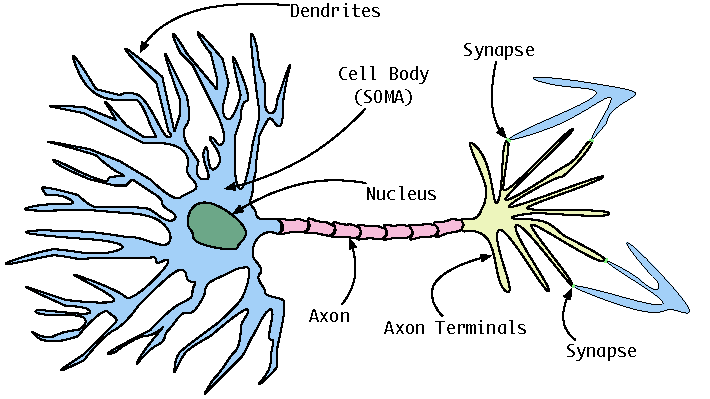
\includegraphics[width=4.0in]{Neuron.pdf}}
}
\caption{Neuron}
\label{fig:neuron}
\end{figure}



\iftrue
So it is known that mammalian neurons generate "spikes" in response to inputs which for humans include sight, touch, sound etc.. This spiking behavior is often referred to as the neuron being activated.
When these neurons are activated, their spikes propagate to other neurons. Under certain conditions, the combination of the various inputs to a neuron cause it to activate. 
A particular neuron may have many hundreds, perhaps thousands of other neurons connected to its "input".
These input neurons are referred to as pre-synaptic neurons. These pre-synaptic neurons may provide input to many neurons which are referred to as post-synaptic neurons.
A particular neuron can get activated by a particular arrival pattern of pre-synaptic neuron spikes or simply by the intensity of the pre-synaptic spikes. 

The spiking behavior of a neuron also varies and many spiking patterns have been observed. 
It is the delays and strength of the connections that contain the "information" in the neural network.
In simple terms, if a neuron is activated by its pre-synaptic neurons, then the activation of the neuron means a pattern has been detected which will influence a reaction.
In mammalian terms, that might be the detection of a threat from both smell and sight neurons and the reaction is to control muscles resulting in flight.

The various chemical and electrical processes that result in the generation and propagation of these neuron spikes is beyond the scope of this dissertation, but how neurons and networks of neurons are artificially emulated is what we will duscuss next.


\subsection*{Artificial Neural Networks}
\label{sec:Artificial Neural Networks}

When modeling these neurons in artificial neural networks, the outputs of the neuron models either generate actual spikes or
produce a value which is proportional to the rate at which spikes occur.
These artificial neural networks can be categorized as rate-based coded or spike time coded neurons.

When used in networks of neurons, both model types employ a connection weight between the pre and post-synaptic neuron, however, the
spiking neuron network also introduces a time delay associated with the connection.
Although the spiking neural network more closely models the behavior of real neurons, over the last 20 years there 
have been breakthroughs in the configuring of rate-based models especially in the application of the back-propagation
algorithm and stochastic gradient descent. Along with the abundance of data now available in the form of voice, images etc. to "teach" these networks
using back-propagation, most of the effective applications of artificial neural networks have employed these rate-based models.
Our research will focus on these rate-based models which we will now refer to as ANNs.
\fi

To approach the capabilities observed in human behavior, such as object recognition these ANNs become very large.
They often utilize hundreds of thousands of neurons to implement what we would consider a relatively straightforward task.
For example, a "useful" ANN similar to that described in \cite{krizhevsky2012imagenet} that is used
to recognize up to 1000 different object classes has a network size of approximately 650,000 neurons and 
630 million synaptic connections \cite{krizhevsky2012imagenetPreso}. 
Many applications require multiple instances of ANNs of similar size to the ANN described in \cite{krizhevsky2012imagenet}.
For example employing multiple cameras in a drone or automobile each with an image recognition ANN\cite{krizhevsky2012imagenet}\cite{bojarski2016end}.
These implementations have very large memory and processing requirements.
The requirements of these applications are typically satisified by employing multiple graphics processor units(GPU).
These multiple GPU systems have high real-estate and power requirements that may exceed the target applications requirements.

This research explores a 3DIC solution using a custom organized 3DIC memory in conjunction with unique data structures and custom processing modules to significantly reduce the 
area and power footprint of an application that needs to support the processing associated with multiple ANNs.


Artificial Neural Networks are a network of inter-connected processing elements inspired by the 
connectivity and processing observed in the brain.
% Uncomment for dissertation

They are characterized by the connections between a pre-synaptic neuron and a post-synaptic
neuron having a weight which determines the impact the pre-synaptic neuron has on the 
"activation" of a post-synaptic neuron.
Typically the processing portion of the neuron performs a multiplication and accumulation on the outputs from all
the pre-synaptic neurons followed by a non-linear "activation" function, such as a rectified linear unit or sigmoid function to create the neuron output.

It is well understood a single layer of these neurons can be configured to perform a linear function approximation.
A collection of these neurons, when connected in layers with one layers neurons connected to
the next layers neurons, are known to be able to act as non-linear function approximators.
As well as being effective function approximators, these neurons can be configured to act as 
classifiers, attractor networks or associative memories.
A simple example of an ANN can be seen in \fref{fig:simpleNetwork} and the contents of an artificial neuron 
with the multiplication and summation stages and the activation function $f(x)$ can be seen in \fref{fig:cellContents}. 


\begin{figure}
\centering
\begin{subfigure}{.65\textwidth}
  \centering
  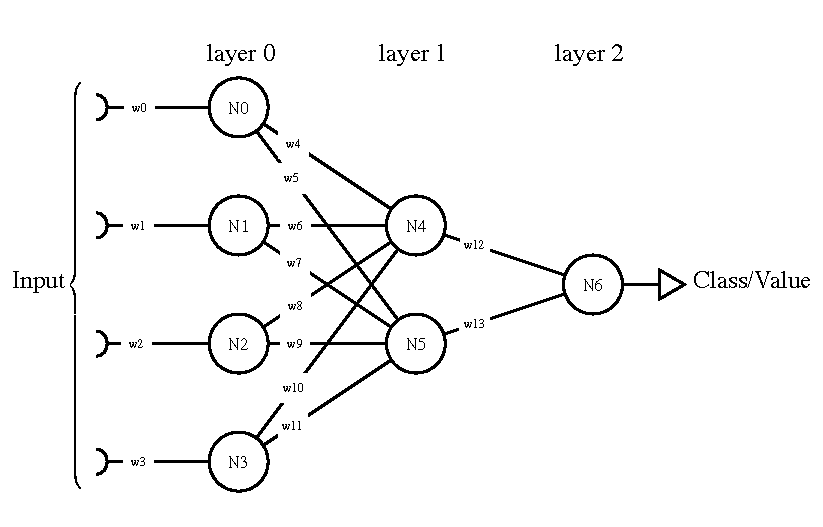
\includegraphics[width=0.9\textwidth]{Chapter-1/figs/simpleANN}
  \captionsetup{justification=centering, skip=-20pt}
  \caption{network}
  \label{fig:simpleNetwork}
\end{subfigure}%
\begin{subfigure}{.3\textwidth}
  \centering
  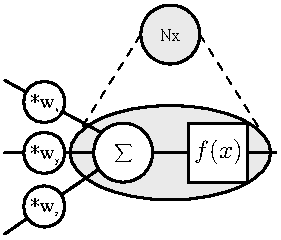
\includegraphics[width=0.7\textwidth]{Chapter-1/figs/cellContents}
  \captionsetup{justification=centering, skip=3pt}
  \caption{neuron}
  \label{fig:cellContents}
\end{subfigure}
\captionsetup{justification=centering, skip=10pt}
\caption{Simple Artificial Neural Network}
\label{fig:Simple Artificial Neural Network}
\end{figure}

For the most part, different ANNs are characterized by the function contained in the
processing element, how the neurons are interconnected and how the weights of the inter-connections are configured or learnt.
Most of the effective applications of ANNs require 10's of thousands of neurons and millions of synaptic connections.
When the entire network must generate a result in near real-time, the result is a system requiring billions
of floating point operations per second. When multiple ANNs need to be processed in parallel, the power and area requirements may not always be satisifed
using current technology.

%%
%%When multiple of these networks must be processed in parallel \cite{qiu2013parallel}\cite{bojarski2016end},
%%we quickly exceed the capabilities of current state-of-the-art technology.
%-------------------------------------------------------------------------------------
% FIXME - do we need activation function figures?
% start FIXME
\iftrue
Some typical examples of the 
activation function can be seen in \fref{fig:Typical neuron activation functions}.

\begin{figure}
\centering
\begin{subfigure}{.32\textwidth}
  \centering
    \begin{tikzpicture}[scale=0.55]
      \begin{axis}[
          xlabel={$$},
          ylabel={$$},
          xlabel style={below right},
          ylabel style={above left},
          title={Sigmoid},
          %grid = major,
          xmin=-6,xmax=6,
          ymin=0,ymax=1,
          legend style={draw=none, fill=white},      
          legend pos= outer north east
          ]
          \addplot[myBlackThickStyle] expression[domain=-6:6,samples=100]{1/(1+e^(-x))} 
                      node at (axis cs:3,0.7){}; 
          %\legend{{\large $f(x)=\frac{1}{1+e^{-t}}$}}
      \end{axis}
    \end{tikzpicture}
  \captionsetup{justification=centering, skip=3pt}
  \caption{Sigmoid}
  \label{fig:SigmoidFunction}
\end{subfigure}%
\begin{subfigure}{.32\textwidth}
  \centering
    \begin{tikzpicture}[scale=0.55, transform shape]
      \begin{axis}[
          xlabel={$$},
          ylabel={$$},
          xlabel style={below right},
          ylabel style={above left},
          title={ReLu},
          xmin=-1,xmax=1,
          ymin=0,ymax=1,
          legend style={draw=none, fill=white},      
          legend pos= outer north east
          ]
           \addplot[myBlackThickStyle] expression[domain=0:1,samples=100]{x} node at (axis cs:0.6,0.15){}; 
           \addplot[myBlackThickStyle] expression[domain=-1:0,samples=100]{0};       
           %\legend  {{ $f(x)= \begin{cases} 0,      &\text{if $x < 0$;}\\   x,       &\text{otherwise.}  \end{cases}$}}  
      \end{axis}
    \end{tikzpicture}
  \captionsetup{justification=centering, skip=3pt}
  \caption{ReLu}
  \label{fig:ReLuFunction}
\end{subfigure}
\begin{subfigure}{.32\textwidth}
  \centering
    \begin{tikzpicture}[scale=0.55]
      \begin{axis}[
          xlabel={$$},
          ylabel={$$},
          xlabel style={below right},
          ylabel style={above left},
          title={Saturation},
          xmin=-2,xmax=2,
          ymin=-1.5,ymax=1.5,
          legend style={draw=none, fill=white},      
          legend pos= outer north east
          ]
           \addplot[myBlackThickStyle] expression[domain=-1:1,samples=100]{x} node at (axis cs:0.6,0.15){}; 
           \addplot[myBlackThickStyle] expression[domain=-2:-1,samples=100]{-1};       
           \addplot[myBlackThickStyle] expression[domain=1:2,samples=100]{1};       
           %\legend  {{ $f(x)= \begin{cases} 1,      &\text{if $x \ge 1$;}\\ x,      &\text{if $-1<x<1$;}\\  -1,      &\text{if $x \le -1$;} \end{cases}$}}  
      \end{axis}
    \end{tikzpicture}
  \captionsetup{justification=centering, skip=3pt}
  \caption{Saturation}
  \label{fig:SaturationFunction}
\end{subfigure}
\captionsetup{justification=centering, skip=3pt}
\caption{Typical neuron activation functions}
\label{fig:Typical neuron activation functions}
\end{figure}

\fi
% end FIXME
%-------------------------------------------------------------------------------------

%%This research will target a family of ANNs that have demonstrated efficacy in
%%a family of popular applications. These applications have large neural networks requiring a large amount of memory 
%%to support weight storage and the requirement of processing multiple ANNs at or near real-time.
% FIXME - should I use this line or a version of it
%As mentioned in section \ref{sec:chap-one}, it is our belief that most useful applications of ANNs fall into this category.

%% Moved to chapter 3
%%\subsection*{Targeted Applications}
%%\label{sec:Targeted Applications}
%%
%%This work will target:
%%\begin{outline}
%%\renewcommand{\outlinei}{enumerate}
%%  \vspace{-3mm}
%%  \1 Brain-state-in-a-Box (BsB) and Cogent Confabulation (CC) because of their demonstrated efficacy in text recognition \cite{qiu2013parallel}.
%%    \vspace{-3mm}
%%    \2 The system described in \cite{qiu2013parallel} utilized 78 clusters with each cluster incorporating 22 Sony PS3 game stations and two NVidia GPU
%%       cards. The text recognition system was segmented into character recognition performed by the BsB networks and the word and sentence construction was
%%       performed by Cogent Confabulation.
%%       There is opportunity to accelerate BsB and potential to accelerate portions of the Cogent Confabulation networks.
%%  \vspace{-08mm}
%%  \1 Deep neural networks \cite{krizhevsky2012imagenet} because of their demonstrated efficacy in image recognition 
%%    \vspace{-3mm}
%%    \2 The application space includes autonomous navigation of automobiles \cite{bojarski2016end}
%%       with a need to process multiple deep neural networks simultaneously at real-time.
%%  \vspace{-3mm}
%%  \1 Reinforcement learning in the context of ANNs
%%    \vspace{-3mm}
%%    \2 The reinforcement learning algorithm employs deep neural networks in action-value function approximation \cite{mnih2013playing}. 
%%       Considering most environments will have very large state spaces,
%%       environment exploration will result in large numbers of action-value calculations and therefore acceleration will improve learning times.
%%       It should be noted that supporting reinforcement learning will require provisions for acceleration of back-propagation.
%%\end{outline}

%%---------------------------------------------------------------------------------------------------------
%%---------------------------------------------------------------------------------------------------------
%% FIXME
%% uncomment for dissertation
\iffalse

\subsubsection*{Brain-State-in-a-Box}

This ANN is an auto-associative memory implemented as a recursive neural network. The network employs the saturation function, shown in \fref{fig:SaturationFunction} 
as its activation function.
The network is trained to a set of attractor primitives as described in \cite{lillo1994synthesis}.
During inference, the network neurons are loaded with the state of the input which is typically a noisy version of one of the stored primitives.
The network is then iteratively processed until the value of each node approaches unity indicating the network has converged on a stored primitive.
The iterative process taking multiple passes through the neural network and that many BsB networks are employed in a given application
provides opportunity for a solution that provide acceleration and large storage.

\fi


\iffalse

\subsubsection*{Cogent Confabulation}

Cogent confabulation is a probabilistic model where the synaptic weight reflects the coexistence likelihood between symbols in different lexicons.
Each neuron represents a specific symbol in a lexicon and the activation value of each neuron is proportional to the co-existence likelihood between
the symbol the neuron represents and other symbols in the observation.

The weights are typically stored in the form of a matrix known as a knowledge base (KB).
What makes this ANN different is that the processing is not deterministic where with most neural networks, all neurons are processed in a regular fashion.
With cogent confabulation only neurons which have links to an observed or inferred symbol are processed.
An example of predicting a symbols likelihood from other observed symbols can be seen in \fref{fig:Cogent confabulation likelihood calculation}.
\begin{figure}[hbtp]
\centering
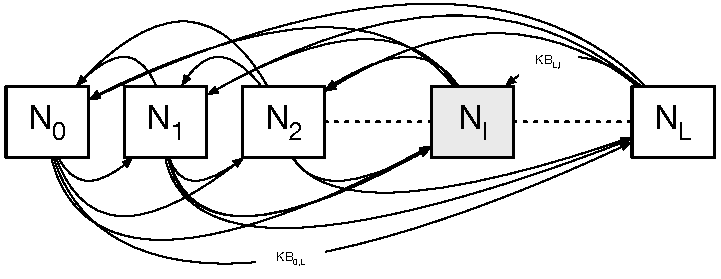
\includegraphics[width=0.4\textwidth]{Chapter-1/figs/CCnetwork}
\captionsetup{justification=centering, skip=3pt}
\caption{Cogent confabulation likelihood calculation}
\label{fig:Cogent confabulation likelihood calculation}
\end{figure}
There is no activation function employed with cogent confabulation neurons.

Cogent confabulation is often used in a process whereby a system converges on the most likely combination of symbols given an obervation \cite{qiu2013parallel}.
It is this converging and the raw size of the knowledge bases that provides opportunity for a solution that provides acceleration and large storage.

\fi


\iftrue

\subsubsection*{Deep Neural Networks}

A single layer of neurons is a linear classifier and therefore cannot be used to classify unless the classes can be separated using a linear function.
Even some simple cases cannot be linearly separated, an example often used is an exclusive-OR gate.
To allow classes in these cases to be linearly separated, the input space needs to be transformed.
Deep neural networks are ANNs that incorporate many layers of neurons which are often up to 10 layers deep.
These additional layers are incorporated to translate the space of the input so the various classes being identified can be separated using linear classifiers in the later
layers.
A very successful early example known as a convolutional neural network (CNN) is which in \cite{krizhevsky2012imagenet} was used to classify objects in images
and shown in \fref{fig:simple Imagenet network}.
\begin{figure}[hbtp]
\centering
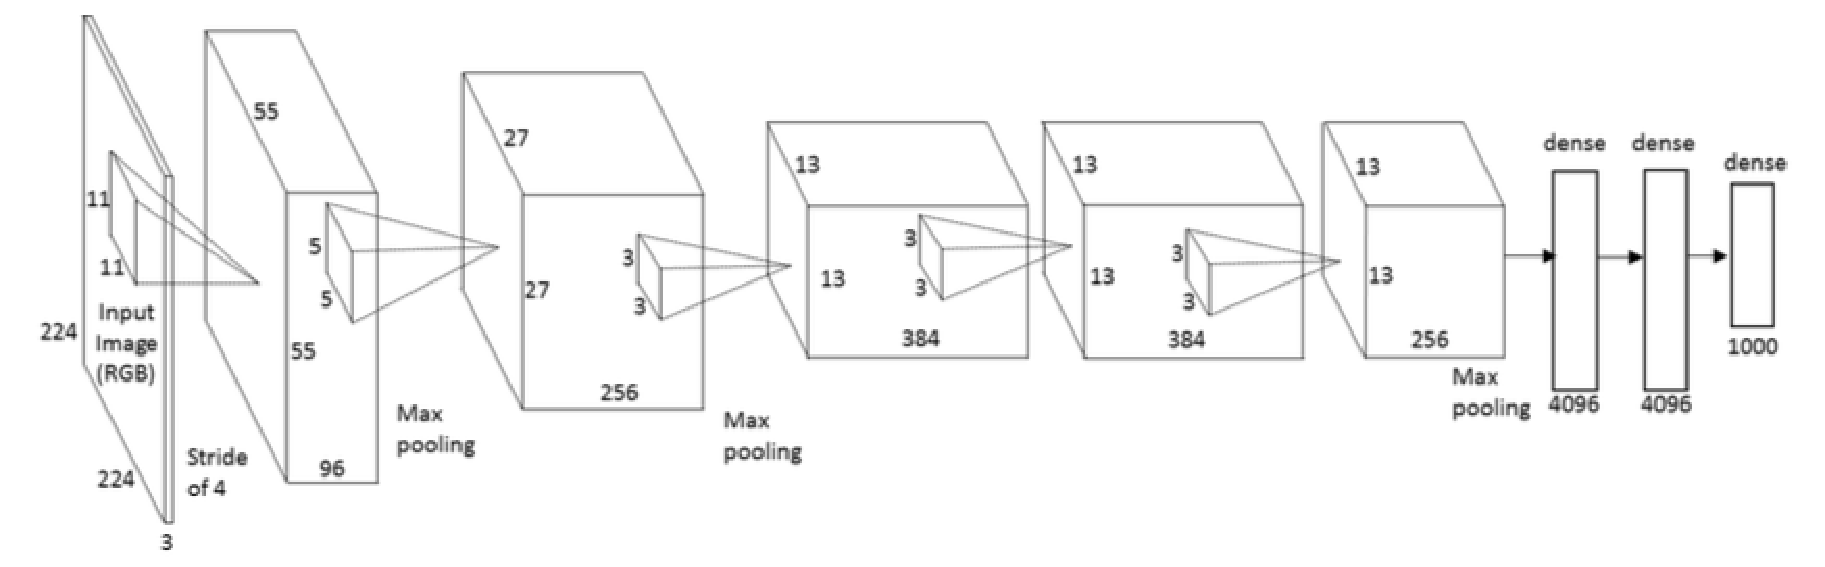
\includegraphics[width=0.9\textwidth]{Chapter-1/figs/deepNetworkShowingFeatureLayers}
\captionsetup{justification=centering, skip=-5pt}
\caption{Imagenet convolutional neural network from \cite{krizhevsky2012imagenetPreso}}
\label{fig:simple Imagenet network}
\end{figure}
These CNN's use the early layers to identify low-level features and later layers are used combine these features into yet more higher-level features.
Finally, the combination of high-level features are used to classify.
This layering is shown in \fref{fig:Deep network showing feature layers}.
\begin{figure}[hbtp]
\centering
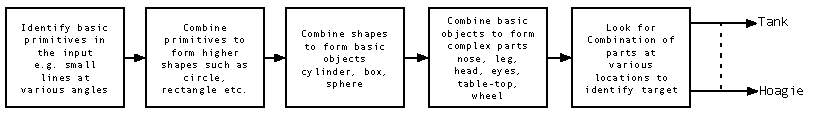
\includegraphics[width=0.8\textwidth]{Chapter-1/figs/deepNetworkBlockDiagram}
\captionsetup{justification=centering, skip=5pt}
\caption{Deep network showing feature layers}
\label{fig:Deep network showing feature layers}
\end{figure}
Finally, a fully connected linear classify is used to classify the object using this translated input.
These deep neural networks can be used as classifiers or as function approximators as in our implementation of reinforcement learning.
In practice, useful deep neural networks are very large and often exceed the capacity of single GPU's. Therefore,  there is opportunity for a solution that provides
real-time acceleration and storage of of these systems.

\fi


\iftrue

\subsubsection*{Reinforcement Learning}
In the context of this work, reinforcement learning is the process by which a system identifies the actions to take to maximize reward.
For example, what actions should an aircraft take to avoid crashing (low reward) versus landing (high reward).
In this context of this work, we are discussing solving the action-reward function associated with a complex Markov-Decision-Process (MDP).
The action-reward function tells an agent operating in an environment the expected accumulated reward if an action is taken
in a particular state. The idea being the agent should always take the action that provides maximum expected reward.
The action-value function is defined for any state an agent may find itself in.
There are various dynamic programming methods employed to "learn" this action-value function and in most cases through repeated trials.
However, in most useful environments, the size of the state-space is too large to learn and/or store each states action-value table, therefore action-value function
approximators are used and deep neural networks are used as these approximators \cite{mnih2013playing}.
The focus of this work will be on accelerating the application of deep NNs to action-value function approximators.

\fi

%%---------------------------------------------------------------------------------------------------------
%%---------------------------------------------------------------------------------------------------------


